\section{Carbon Intensity Prediction}
\noindent

Understanding and predicting the carbon intensity is crucial in assessing the environmental impact and in the development of regulatory policies. 
Therefore, the usage of prediction of future carbon intensity is very crucial to mitigate its effects in peak periods. 
The distribution of the available data on carbon intensity (CI) is in the range of 3 years from January 2021 to January 2024 \cite{ElectricityMap}. 
Analysis of the data demonstrates the seasonality, which makes the data generally predictable. 

\begin{figure}[H]
    \centering
    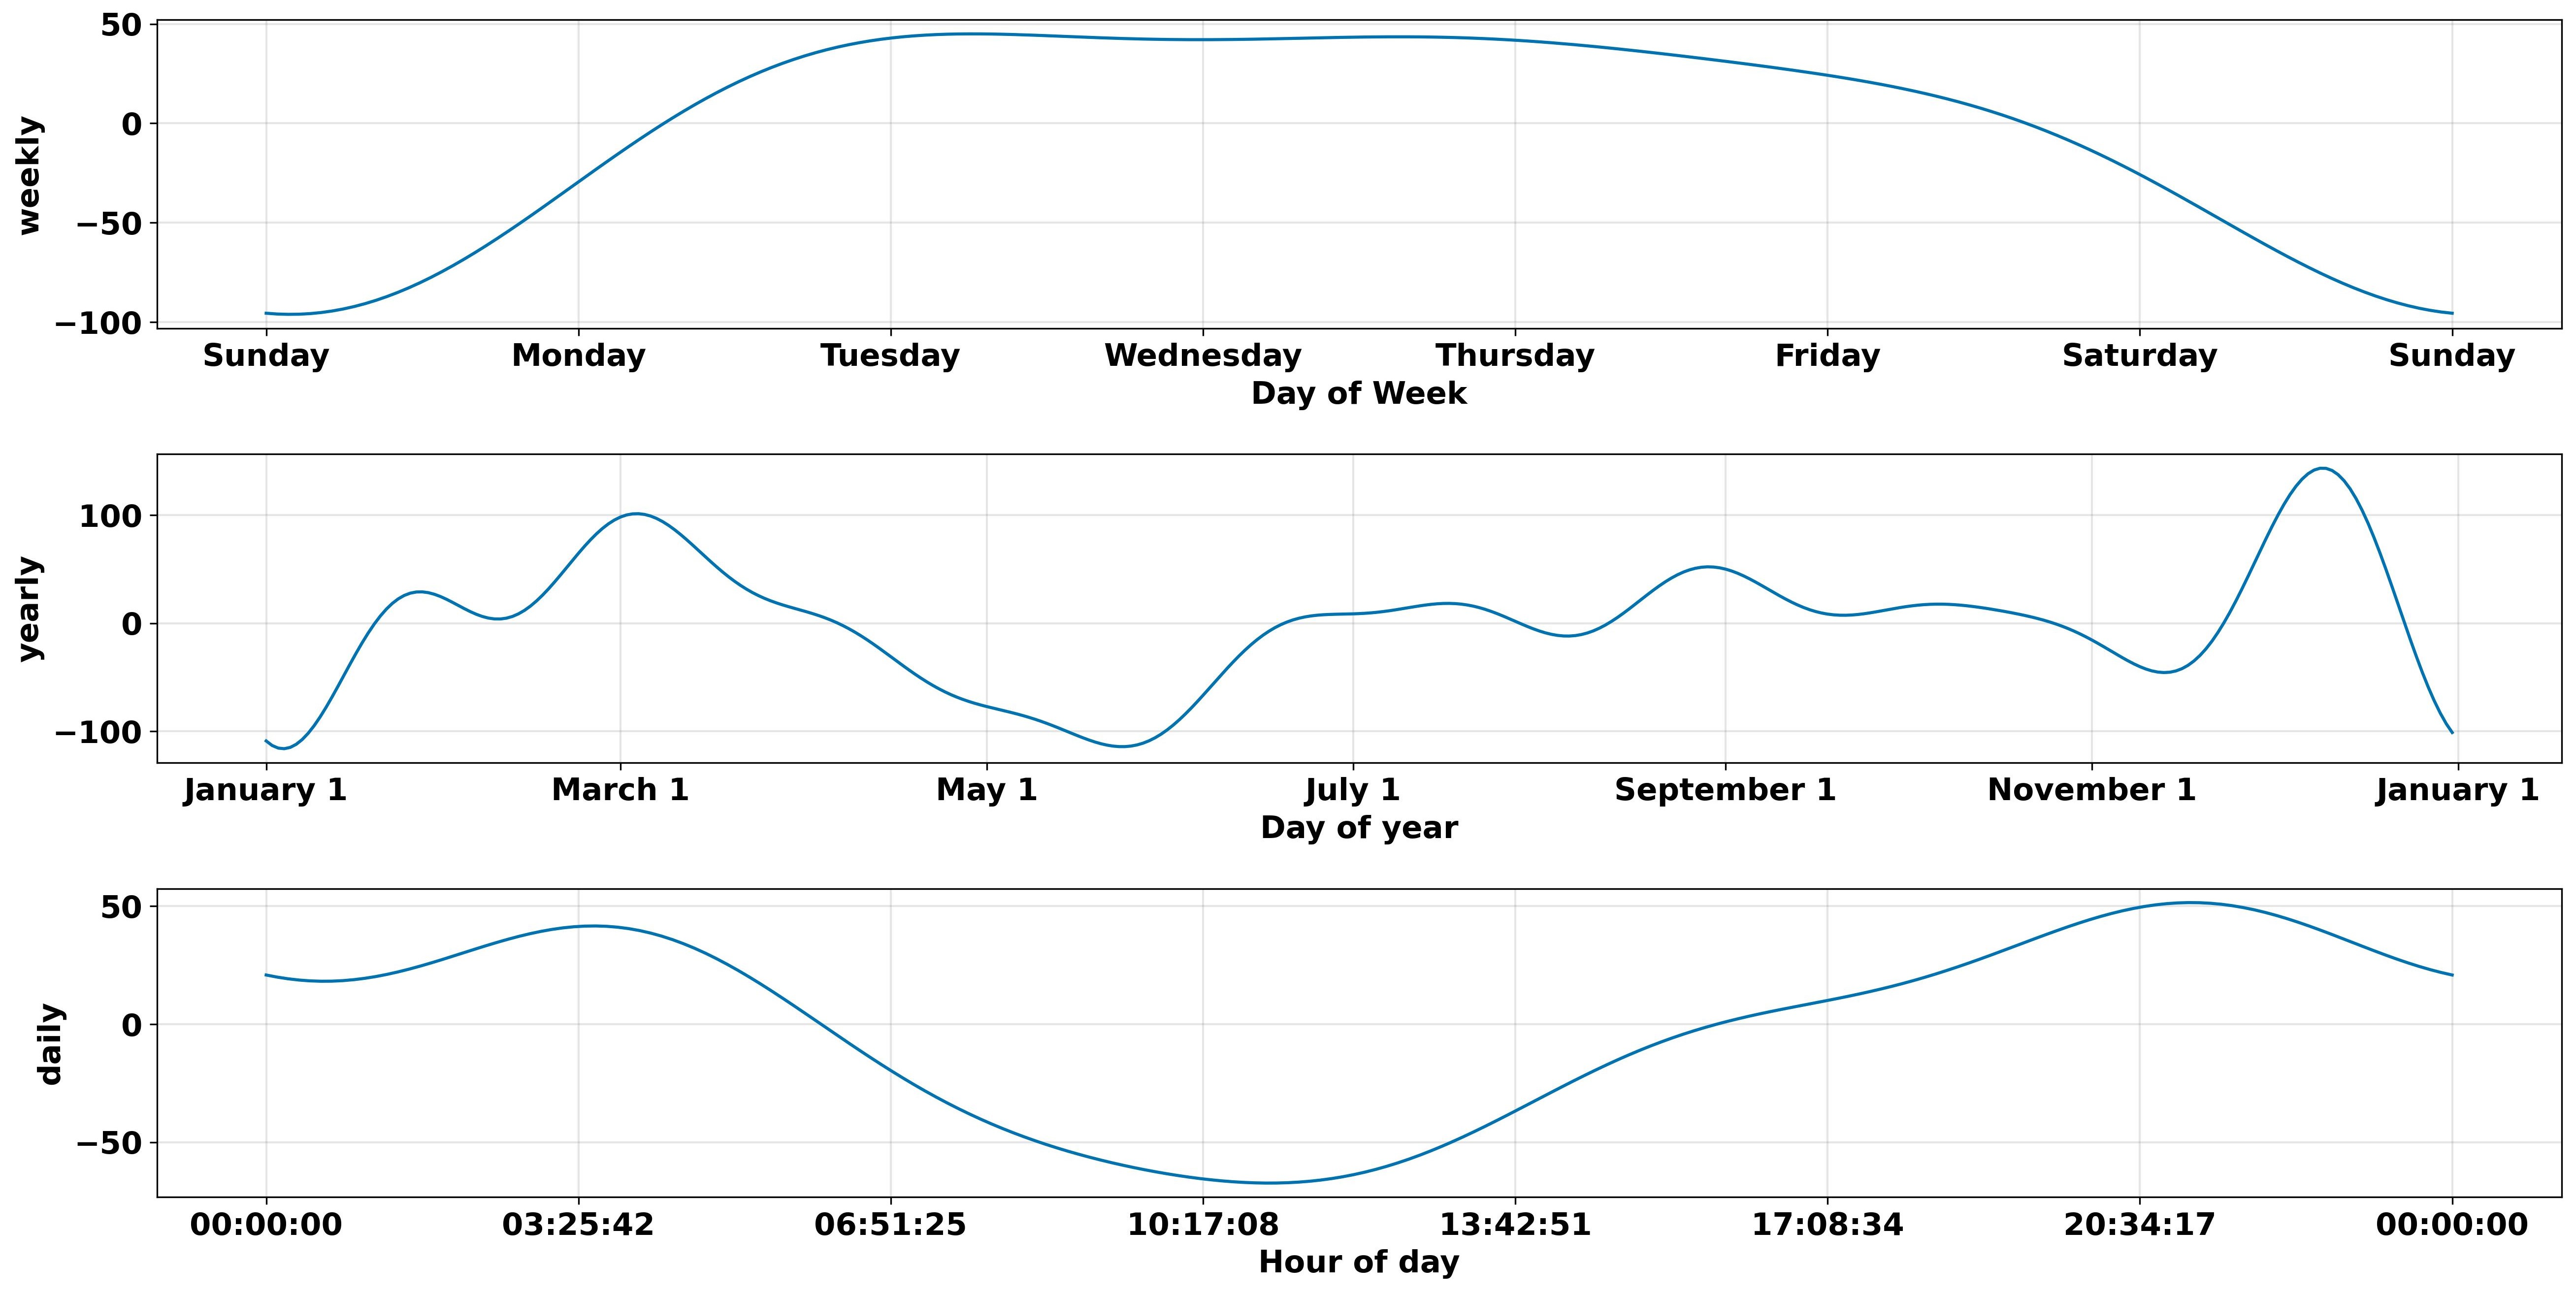
\includegraphics[width=1\textwidth]{Figures/CI_seasonality.jpg}
    \caption{Carbon Intensity seasonality}
    \label{fig:CI_seasonality}
\end{figure}

\begin{figure}[H]
    \centering
    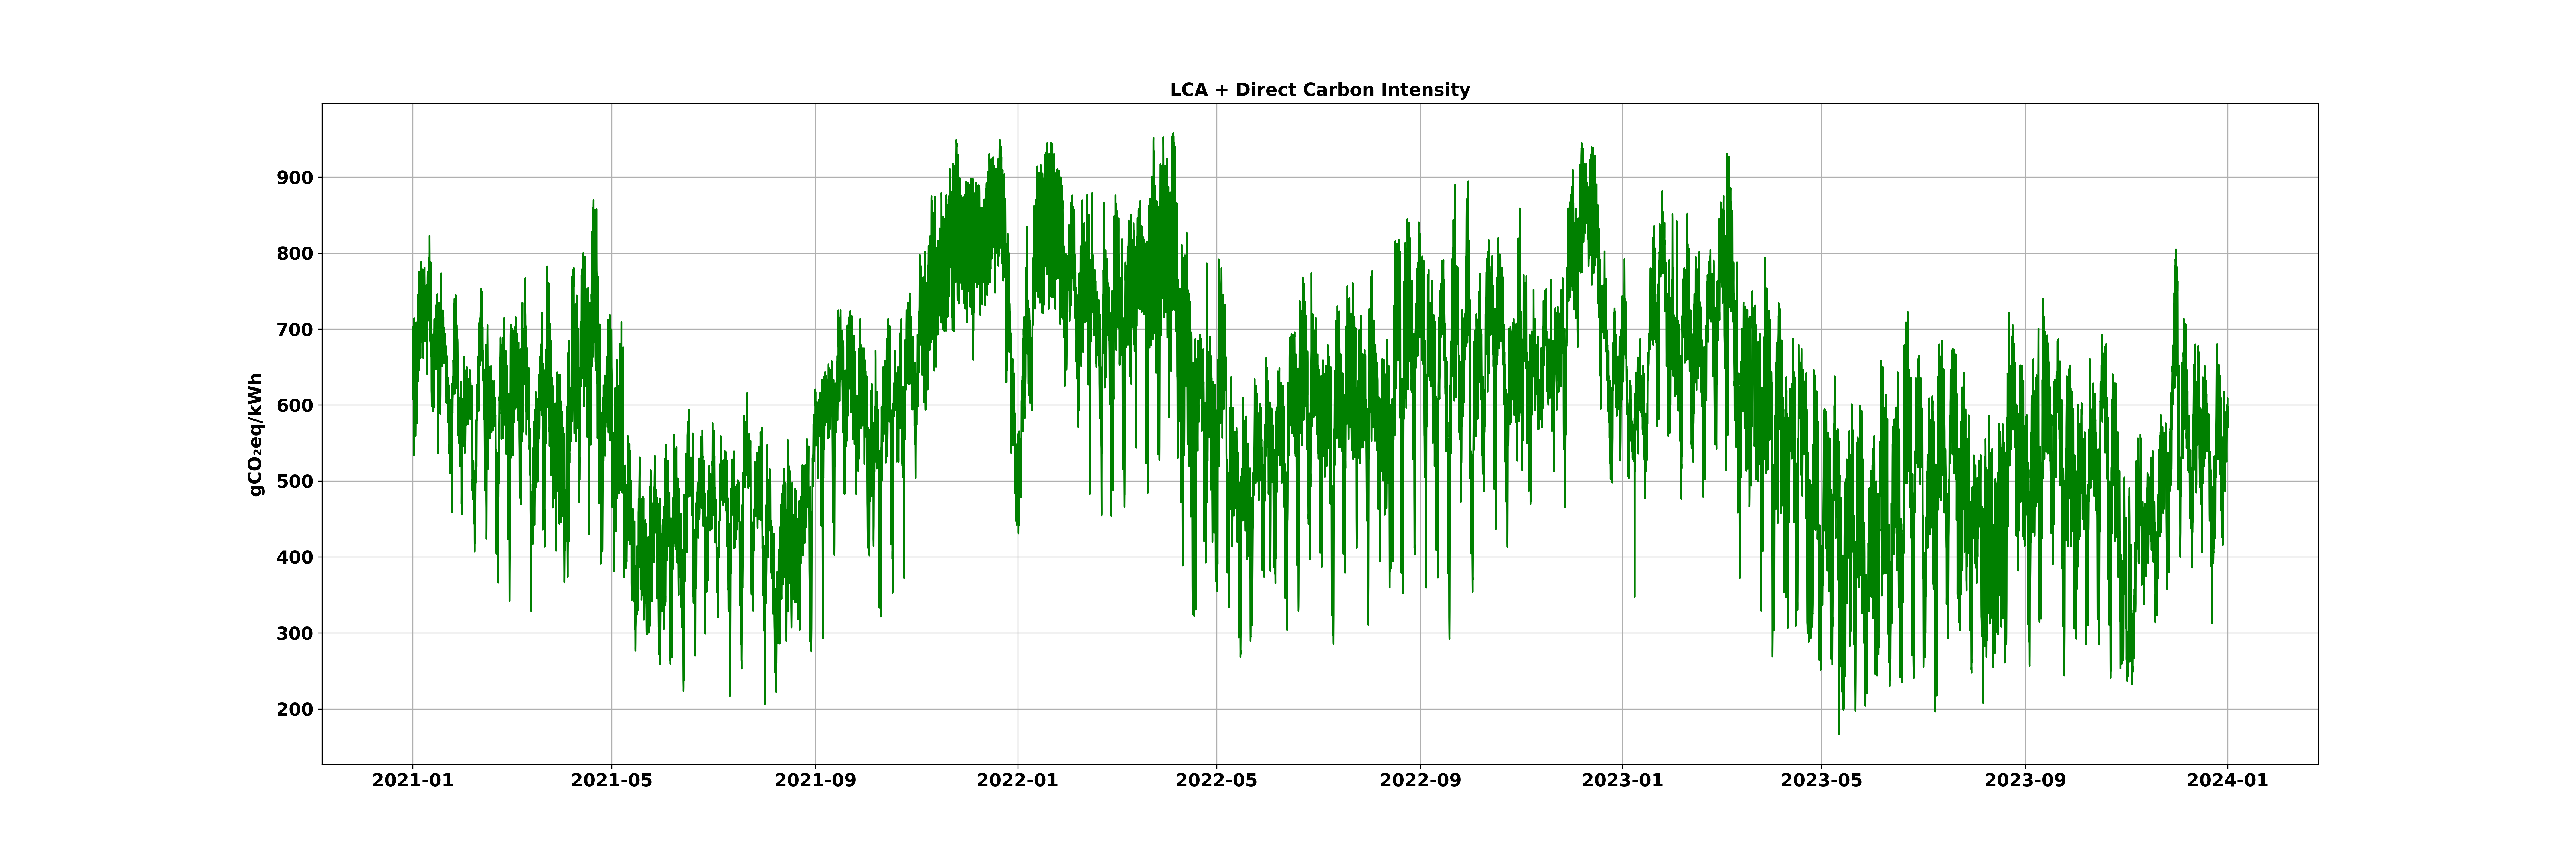
\includegraphics[width=1\textwidth]{Figures/CI_LCA+direct.png}
    \caption{Carbon Intensity LCA + direct}
    \label{fig:CI_LCA+direct}
\end{figure}

As it can be seen from the visualization, the data has a periodicity which is useful in the prediction of future behavior. 
The periodicity depends on many factors, for example, the most impactful of the effects is the difference in CI as of summer (hotter periods) and winter (colder periods), as well as the variation during the week - working days demonstrate higher CI, compared to weekend. 
Moreover, throughout the day the carbon intensity is higher during business hours. 
Hence, by analyzing these patterns we can predict the future CI, and evaluate its accuracy. 

\subsection{Prediction Techniques of CI}
The methodology for our prediction is based on a comparison of two models: the baseline last value predictor, and the machine learning (ML) model. 
The first, simple baseline model is the prediction based on the previous observed value: the next value is dependent on the last week’s value at the same time and week of the day. 
The advantage of this prediction is that it is generally a lightweight solution requiring minimal computational resources, however, it has no extended parameter tuning options. 
The second, ML model is based on the Prophet time series predictor, which is a more complex solution compared to the first one. 
ML models can capture the patterns and relationships in data points, as well as adapt to the changes in data distribution, being more robust with dynamic data. 
Hence, using such a lightweight solution in comparison with a complex ML model allows us to compare the efficiency of the predictive ML model. 
\\
Our ML model is the Meta’s Prophet time series predictor, which is a powerful tool for predicting the time series. 
To achieve the best performance, we trained the predictor on different periods of the dataset, particularly, from 30-month data to 10 months with a step of 2 months, which demonstrated the impact of historical data. 
Furthermore, we compared the performance on varying lengths of the forecasting horizon. 
Moreover, based on the prophet documentation, the available hyperparameters were tuned to find the best-performing configuration. 

\subsection{Prediction Result}
Based on our prediction using the last value predictor, it has demonstrated an absolute error of 16.22\% \ref{fig:CI_PRED}. 
On the same dataset, our ML model has been trained on 130 different possible configurations of parameters, which resulted in the error rate in a wide range of 10\% to 159\%. 
Particularly, as a result of the tuning ML prediction, our key finding demonstrates that we could achieve the 10.31\% absolute error relative to the real data with training on 16 month period and prediction horizon for 2 months with the parameters of '\textit{changepoint_prior_scale}' as 0.1, and '\textit{seasonality_prior_scale}' as 0.01. 
The first parameter controls the flexibility of the trend by adjusting the penalty for changepoints in the time series trend, adding more flexibility to fit small fluctuations, while the second parameter controls the "strength" of the historical distribution over the prediction. 
Therefore, we could surpass the simple model prediction using the ML approach. 

\begin{figure}[H]
    \centering
    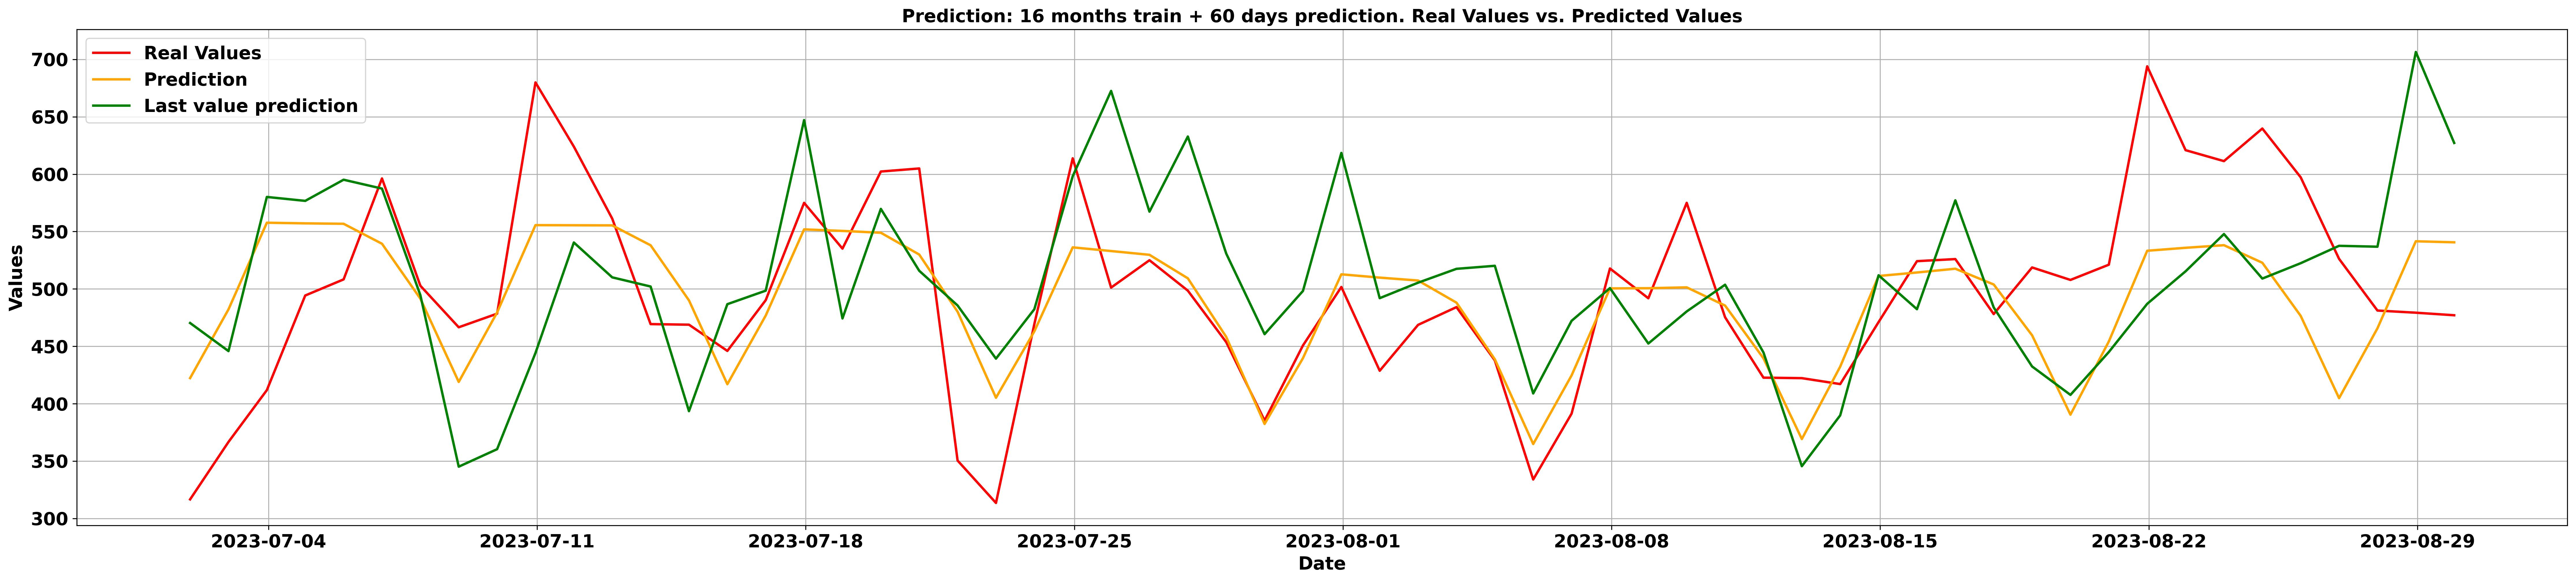
\includegraphics[width=1\textwidth]{Figures/CI_PRED.jpg}
    \caption{Carbon Intensity prediction}
    \label{fig:CI_PRED}
\end{figure}

Generally, the usage of the prediction technique helps us to estimate future CI behavior to develop policies toward reducing it. In the context of heavy computational tasks, such models can utilize real-time monitoring of CI levels, allowing the possible implementation of task scheduling techniques in off-peak CI hours, reducing overall the carbon footprint and, hence, the environmental impact.  